%!TEX root = 0_architecture_rapport.tex

% subsection title
\section*{Question 4}
\addcontentsline{toc}{section}{Question 4}
\label{subsec:3Q4}

\paragraph{Upper-bound or lower-bound coefficients}We use the best model we have, i.e. the model with the points, rebounds and assists. 
We first plot the standard error between the estimate salary and the real salary, with the real salary on the x axis. We can see that our prediction is not very good for low salaries but rather good for high salaries (even if it is normal that the standard error diminishes when the salary increases).
\begin{figure}[h!]
\centering
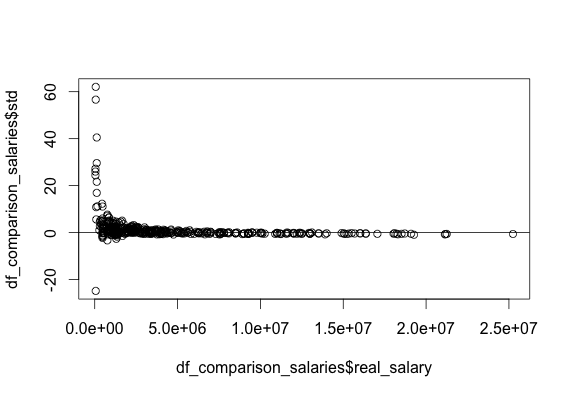
\includegraphics[width=0.75\textwidth]{images/Std_error}
\end{figure}
\\
We then plot the estimate salaries with the real salaries on the x axis. We can see that the coefficients we predicted are upper-bound for low salaries and lower-bound for high salaries.
\begin{figure}[h!]
\centering
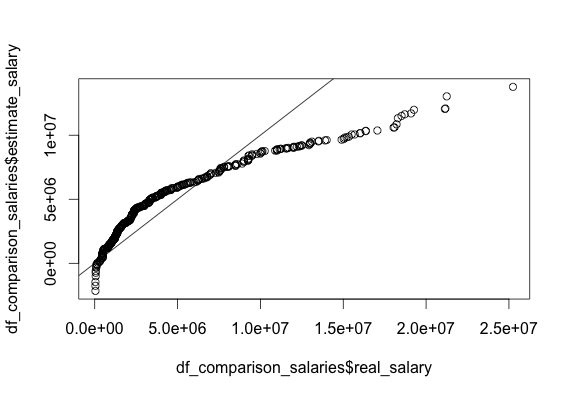
\includegraphics[width=0.75\textwidth]{images/Estimate_salaries}
\end{figure}
